
\documentclass[12pt]{article}
\usepackage{geometry} 
\usepackage{setspace}
\usepackage[italian]{babel}
\usepackage[utf8]{inputenc}
\usepackage{color}
\usepackage{indentfirst}
\usepackage{listings}
\usepackage{graphicx}
\usepackage[dvipsnames]{xcolor}

\geometry{a4paper} 

\lstnewenvironment{codice}
{\lstset{basicstyle=\ttfamily, columns=fullflexible,
keywordstyle=\color{ForestGreen}\bfseries, commentstyle=\color{MidnightBlue}, stringstyle=\color{BrickRed},
language=Python,
numbers=left, numberstyle=\tiny,
stepnumber=2, numbersep=5pt, frame=single,breaklines=True}}{}

\title{\textbf{EasYE TRACKING}}
\author{Giada Colella \and Chiara Coletti}
\date{15/07/2016} 


\begin{document}
	

\begin{figure}
\centering
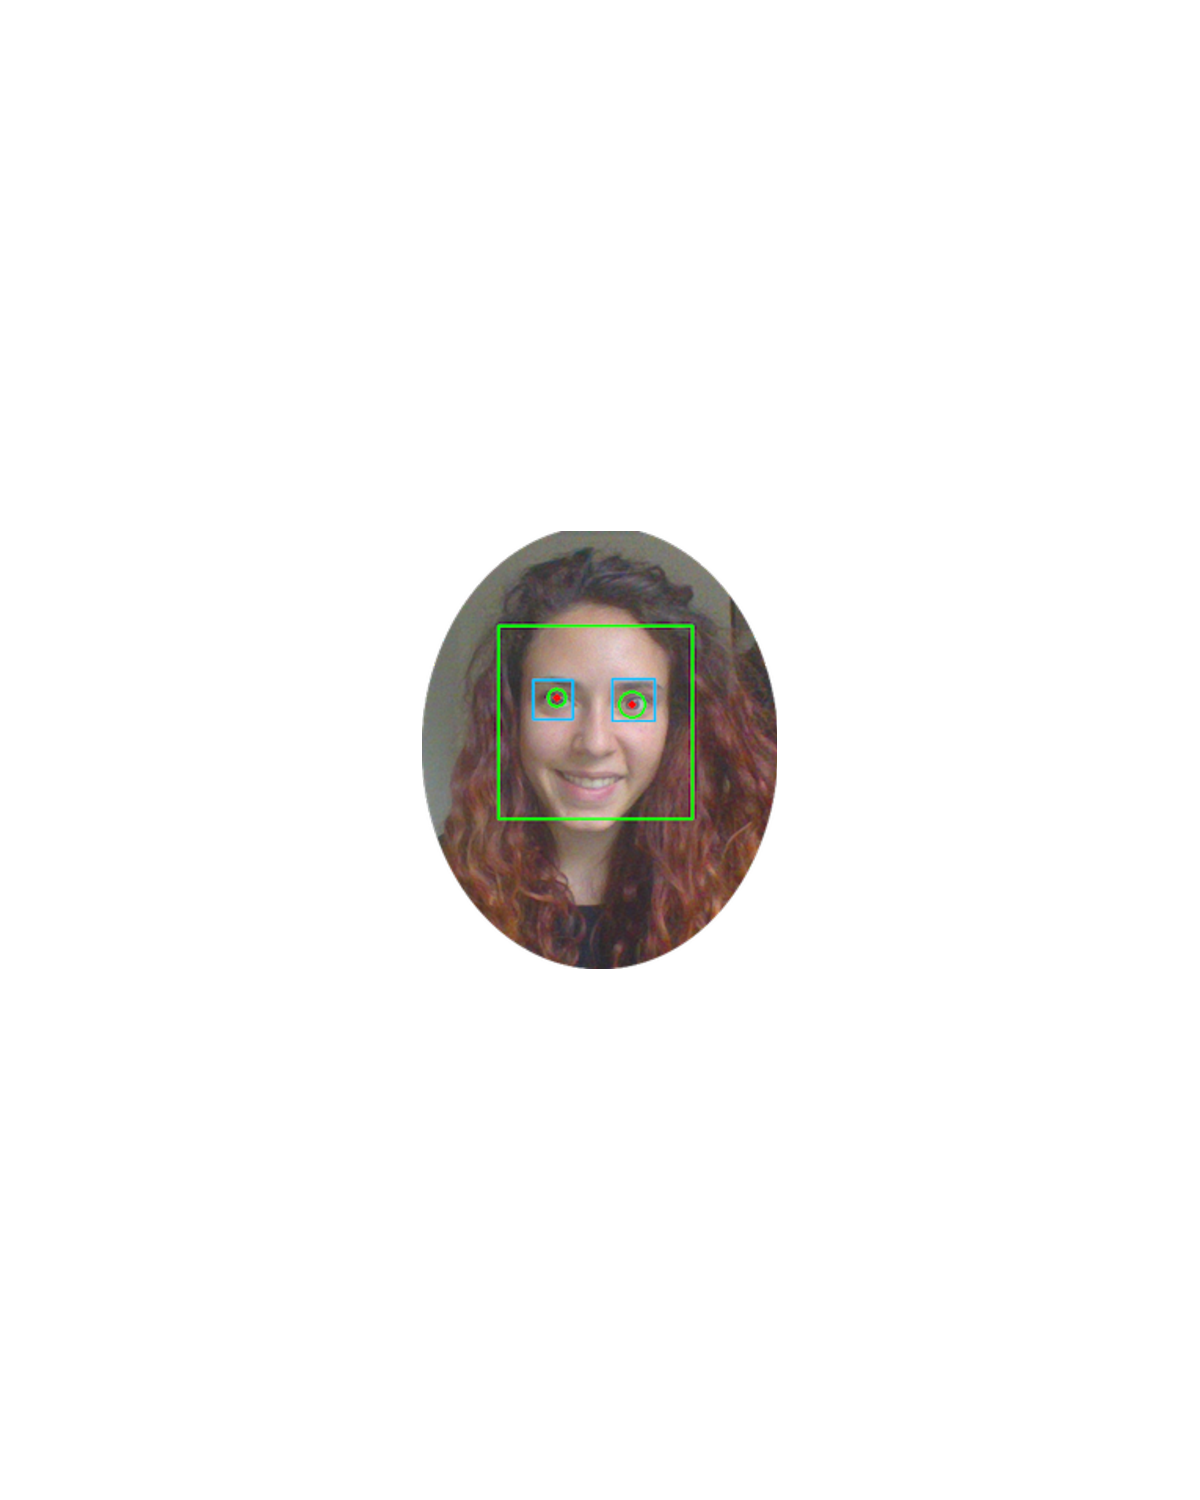
\includegraphics[width=6cm,height=7.2cm]{im2}%
\qquad\qquad
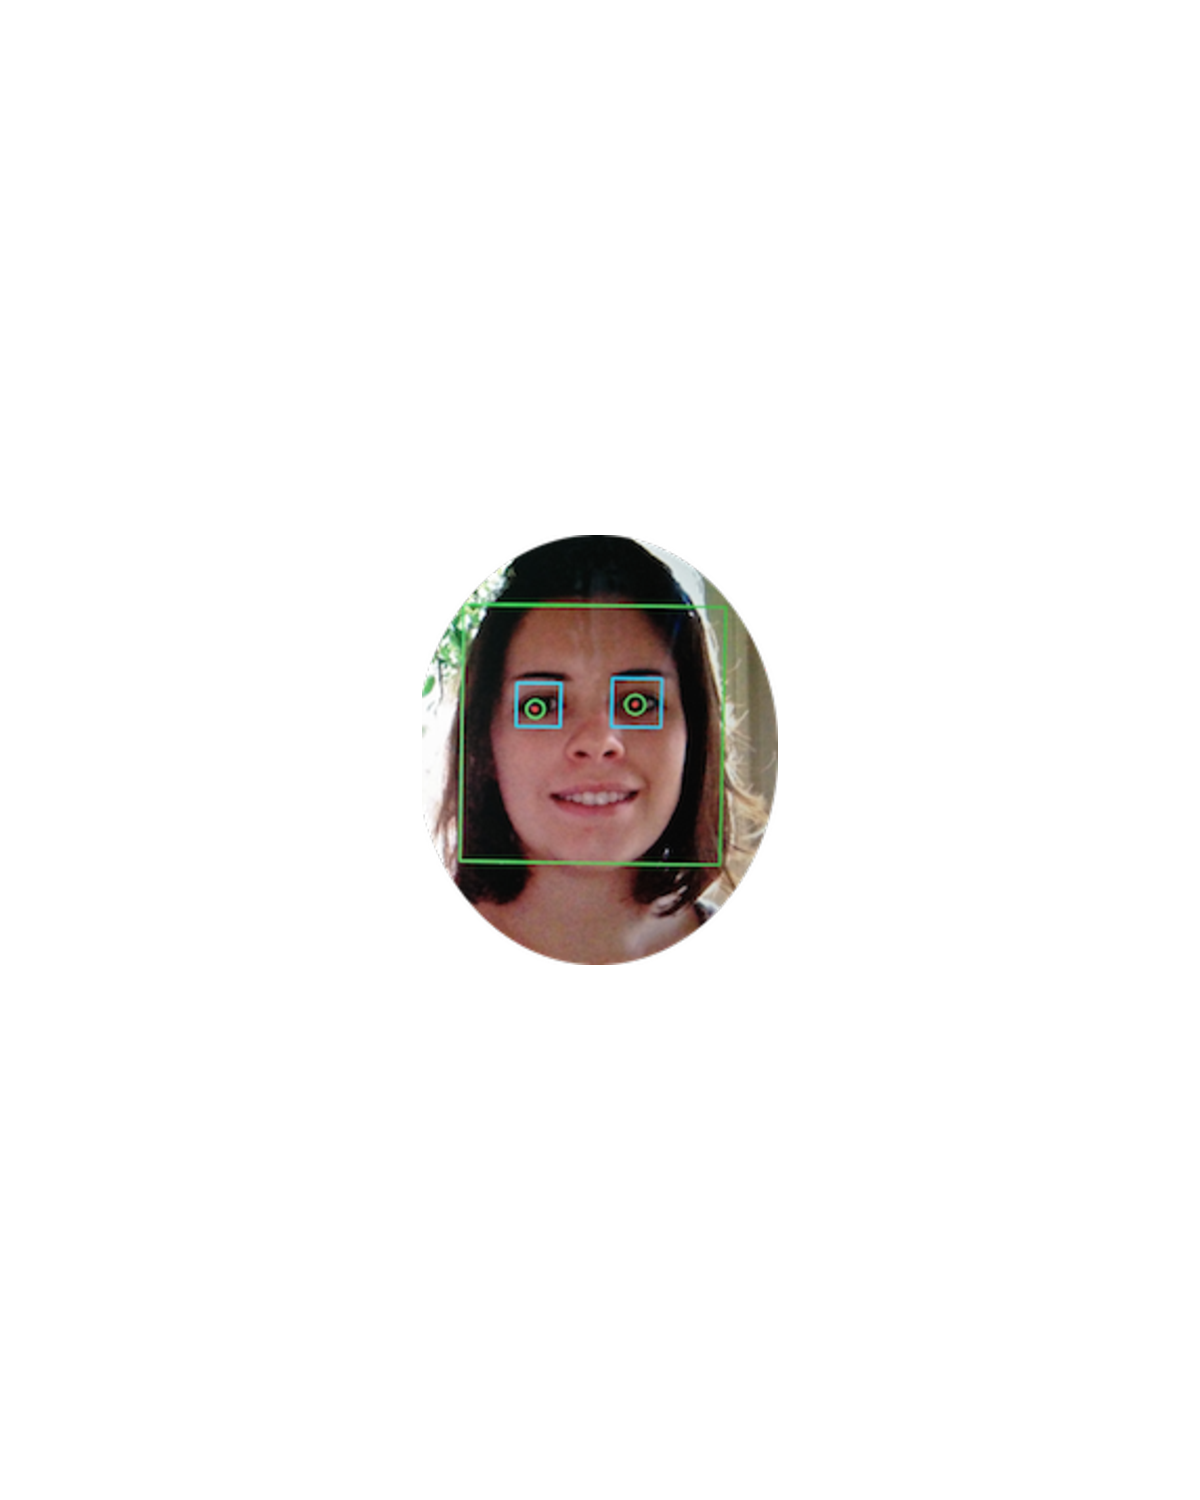
\includegraphics[width=6.1cm,height=7.25cm]{im}
\end{figure}

\maketitle
\pagebreak

\tableofcontents

\pagebreak

\begin{abstract}
	L' Eye tracking è un complesso processo di misurazione del punto di fissazione oculare. I vantaggi che derivano dall'utilizzo di questa tecnica sono molteplici: a partire da indagini statistiche di mercato fino al miglioramento della comunicazione uomo/macchina.
\end{abstract}
\pagebreak
\section{Introduzione}
Il nostro progetto si pone nella prima fase di realizzazione di un eye tracker. Ha come scopo lo studio del movimento dell'occhio. Partendo da un video, abbiamo cercato di individuare l'occhio e di tracciarne il movimento. Punto focale della nostra ricerca è stato il riconoscimento del centro dell'iride. 

Abbiamo sviluppato il nostro progetto usando {\textbf{"Python"} come linguaggio di programmazione. Per iniziare è necessario aver installato la libreria libera Opencv. Il riconoscimento di volti ed occhi è stato realizzato mediante l'algoritmo "Cascade Classification". Prima di operare, dunque, è stato necessario importare i file classificatori (o "haarcascades") nella cartella di lavoro.
\pagebreak

\section{Dallo Pseudocodice...}
Abbiamo ritenuto utile suddividere il nostro progetto in vari step:
\begin{enumerate}
	\item \label{primo}\textcolor{Plum}{Acquisizione video e analisi frame by frame}
	\item \label{secondo} \textcolor{Plum}{Conversione dei frame acquisiti in scala di grigi}
	\item \label{terzo} \textcolor{Plum}{Riconoscimento del volto}
	\item \label{quarto}\textcolor{Plum}{Riconoscimento degli occhi}
    \item \label{quinto}\textcolor{Plum}{Riconoscimento cerchi nell'area occhi}
    \item \label{sesto}\textcolor{Plum}{Rappresentazione del movimento oculare}
    \item \label{settimo}\textcolor{Plum}{Generazione video e chiusura programma}
\end{enumerate}

\pagebreak
\section{...Al codice}
\begin{codice}
%matplotlib inline
import matplotlib.pyplot as plt
import cv2
import numpy as np

sc_fct = 1.1              
min_neigh = 5             
min_size_f = (30,30)      
min_size_e = (10,10)        
mindist_c=30               
dp_c=1                   
param1_c=60               
param2_c=20              
minr_c=5                
maxr_c=15                 


faceCascade = cv2.CascadeClassifier("haarcascade_frontalface_default.xml")
eyeCascade=cv2.CascadeClassifier("haarcascade_eye.xml")
\end{codice}
\vspace{1cm}
Importiamo le librerie oportune, introduciamo i parametri che ci torneranno utili nella stesura del codice ed importiamo le Haarcascades che userem per il riconoscimento di volto e occhi.
\vspace{1.5cm}



\ref {primo} \underline{\textbf{\textcolor{Plum}{Acquisizione video e analisi frame by frame}}}
    \\
    \\
    \\
    \\
    \begin{codice}
video_capture = cv2.VideoCapture(0)
cv2.namedWindow("Face and eyes")
    
while True:
    ret, frame = video_capture.read()
    \end{codice}
    \vspace{1cm}
    
    
    	Abbiamo importato il video dalla webcam, rinominato la finestra video e salvato in "frame" gli elementi su cui poi andremo a lavorare. L'ultima operazione vine inserita all'interno di un ciclo while che verrà interrotto solo al termine dell'esecuzione dell'intero programma.
	\\
	\\
	\\
	\\
\begin{codice}
x_dim=video_capture.get(3)
y_dim=video_capture.get(4)
\end{codice}
\vspace{1cm}
		
Definisco x\_dim e y\_dim come le dimensioni del video in entrata. Saranno utili in seguito.
\vspace{1.5cm}
  
  
\ref {secondo} \underline{\textbf{\textcolor{Plum}{Conversione dei frame acquisiti in scala di grigi}}}
   \\
   \\
   \\
\begin{codice}
	gray = cv2.cvtColor(frame, cv2.COLOR_BGR2GRAY)
\end{codice}
\vspace{1cm}
   
   
     	Applichiamo la funzione 'cvtColor' specificando il tipo di conversione da eseguire (in questo caso convertiamo da una figura a colori ad una a scala di grigi mediante il comando cv2.COLOR\_BGR2GRAY). La funzione viene applicata a 'frame' ovvero la zona di memoria in cui vengono salvati i singoli frame del video.
 \vspace{1.5cm} 	
  	
  
\ref {terzo} \underline{\textbf{\textcolor{Plum}{Riconoscimento del volto}}}
    \\
    \\
    \\

\begin{codice}
    faces = faceCascade.detectMultiScale(       
        gray,
        scaleFactor=sc_fct,
        minNeighbors=min_neigh,
        minSize=min_size_f
        )
\end{codice}
\vspace{1cm}
  
  	Applichiamo la funzione 'detectMultiscale' e utilizziamo le cascaspecificando il tipo di conversione da eseguire (in questo caso convertiamo da una figura a colori ad una a scala di grigi mediante il comando cv2.COLOR\_BGR2GRAY). La funzione viene applicata a 'gray' ovvero la zona di memoria in cui abbiamo salvato i risultati della conversione dei vari frame in scala di grigi. Salviamo l'output della funzione (una lista di quattro elementi: coordinata x e coordinata y del vertice superiore sinistro del rettangolo, base e altezza) in "faces".
  	\\
  	\\
  	\\
  	\\
 \begin{codice}
    for (x, y, w, h) in faces:
            cv2.rectangle(frame,(x, y), (x+w, y+h), (0, 255, 0), 2)
\end{codice}
\vspace{1cm}
	  
	  Tracciamo i rettangoli attorno ai volti riconosciuti mediante la funzione 'rectangle'.
\vspace{1.5cm}	  	
  	
\ref {quarto} \underline{\textbf{\textcolor{Plum}{Riconoscimento degli occhi}}}
  	\\
  	\\
  	\\
  	\\ 
 \begin{codice}
            roi_gray=gray[y:y+h/2,x:x+w]
            roi_color=frame[y:y+h/2,x:x+w]

\end{codice}
\vspace{1cm}
 
    Definisco nuove aree di lavoro: rappresentano la stessa area (limitata alla metà superiore del volto), la prima è in scala di grigi, la seconda a colori.
    \\
    \\
    \\
    \\
 \begin{codice}
             eyes= eyeCascade.detectMultiScale(         
                 roi_gray,
                 scaleFactor=sc_fct,
                 minNeighbors=min_neigh,
                 minSize=min_size_e
                 )  
 \end{codice}
\vspace{1cm}
  
  
  Applichiamo nuovamente la funzione 'detectMultiscale'. Questa volta la funzione viene applicata a 'roi\_gray'.Salviamo l'output della funzione in "eyes".
  	\\
  	\\
  	\\
  	\\
 \begin{codice}
            for (ex, ey, ew, eh) in eyes:
                cv2.rectangle(roi_color, (ex, ey), (ex+ew, ey+eh), (255, 191, 0), 2)
\end{codice}
\vspace{1cm}
 
   	Tracciamo i rettangoli attorno agli occhi riconosciuti mediante la funzione 'rectangle'.
\vspace{1.5cm}
  	 	
 \ref {quinto} \underline{\textbf{\textcolor{Plum}{Riconoscimento cerchi nell'area occhi}}}
  	\\
  	\\
  	\\
  	\\
 \begin{codice}
                roi_gray2=roi_gray[ey:ey+eh,ex:ex+ew]
                roi_color2=roi_color[ey:ey+eh,ex:ex+ew]

\end{codice}
\vspace{1cm} 	
 
 
   	Definisco nuove aree di lavoro: rappresentano la stessa area (limitata ai rettangoli degli occhi riconosciuti), la prima è in scala di grigi, la seconda a colori.
  	\\
  	\\
  	\\
  	\\
\begin{codice}
                circles = cv2.HoughCircles(roi_gray2,cv2.HOUGH_GRADIENT,dp=dp_c,minDist=mindist_c,
                            param1=param1_c,param2=param2_c,minRadius=minr_c,maxRadius=maxr_c)

\end{codice}
\vspace{1cm}

	 Applichiamo la funzione 'HoughCircles' per il riconoscimento degli occhi nell'area inserita come input (roi\_gray2). Salviamo l'output della funzione (una lista di tre elementi: coordinata x, coordinata  e raggio del cerchio riconosciuto) in "circles".
  	\\
  	\\
  	\\
  	\\
\begin{codice}
                if(circles==None):
                    continue
                else:
                     circles = np.uint16(np.around(circles[0,:]))
\end{codice}
\vspace{1cm}

  	 Introduciamo la condizione che ci permette di "bypassare" i frame in cui non viene riconosciuto alcun cerchio. Nel caso in cui, invece, il cerchio venga riconosciuto, 'circles' viene trasformato in un ato di tipo intero.
  	\\
  	\\
  	\\
  	\\
 \begin{codice}
                  for (x_c,y_c,r) in circles:
                    cv2.circle(roi_color2,(x_c,y_c),r,(0,255,0),2)
                    cv2.circle(roi_color2,(x_c,y_c),2,(0,0,255),3)
\end{codice}
\vspace{1cm}
 
 	Tracciamo i cerchi e il loro centro.
  \vspace{1.5cm}	 				
  	 				
  	 				
  	 				
\ref {sesto} \underline{\textbf{\textcolor{Plum}{Rappresentazione del movimento oculare}}}
  	\\
  	\\
  	\\
  	\\
\begin{codice}
                    plt.scatter(x+ex+x_c,y+ey+y_c, s=100, c='r',alpha=0.3)
                    plt.axis([0,x_dim,0,y_dim])
                    plt.draw()
\end{codice}
\vspace{1cm}


  	Introduco uno scatterplot di dimensioni (x\_dim e y\_dim) pari alle dimensioni del video in cui visualizzo il centro di cerchio trovato. I punti hanno una trasparenza tale da permettere di osservare le zone dello scatterplot più dense di punti: ovvero quelle zone in cui lo il centro dell'iride è stato più presente. Si ottiene un output di questo tipo:
\\
\\

\begin{figure}[htbp]
\centering
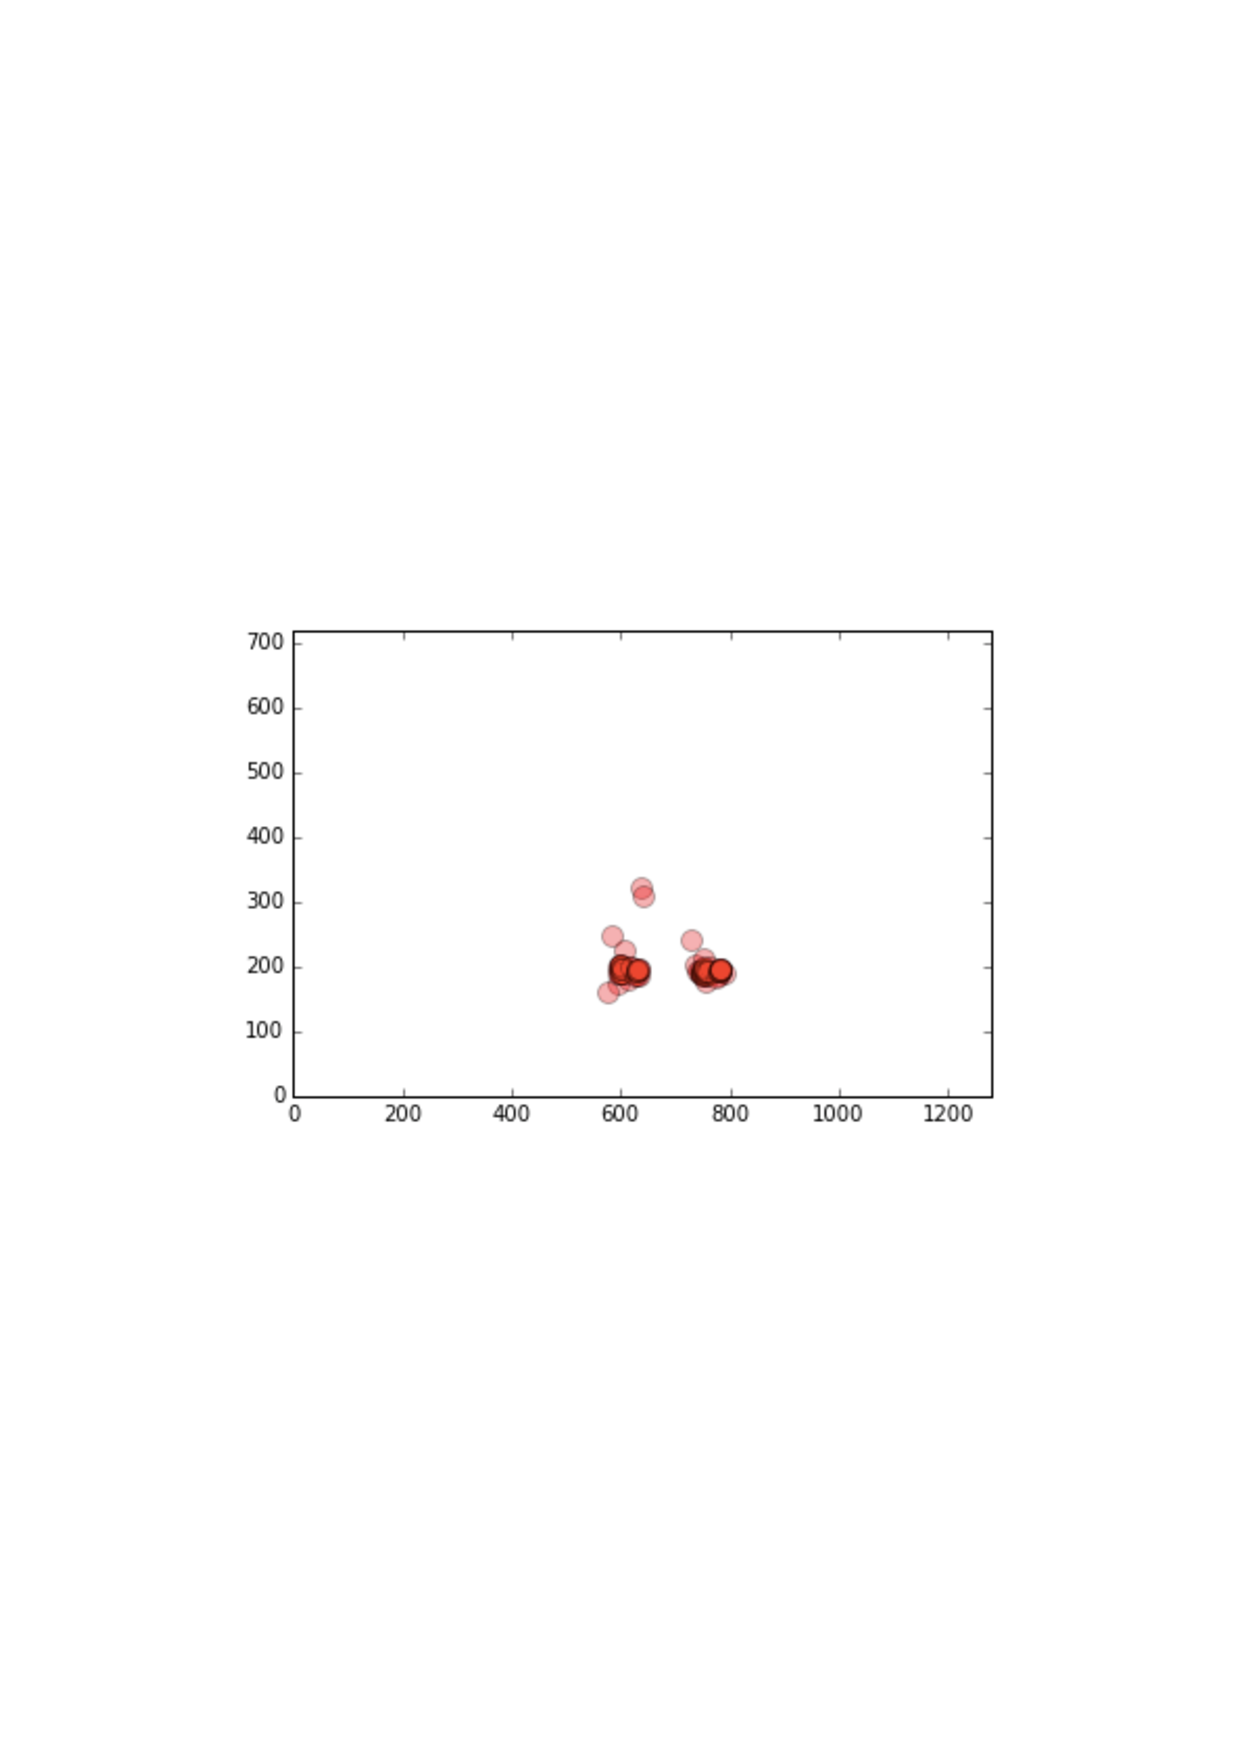
\includegraphics{scatter}
\caption{Esempio scatterplot}
\end{figure}
\vspace{1cm}


\ref {settimo} \underline{\textbf{\textcolor{Plum}{Generazione video e chiusura programma}}}
   \\
   \\
   \\
   \\
 \begin{codice}
    cv2.imshow('Face and eyes', frame)
\end{codice}
\vspace{1cm}
 
    Mostriamo il video. In 'frame' saranno state apportate le modifiche delle varie aree di interesse. Nel video saranno dinque mostrati i rettangoli dei volti e degli occhi riconosciuti e i cerchi trovati all'interno dei rettangoli degli occhi.
   \\
   \\
   \\
   \\
\begin{codice}
    if cv2.waitKey(1)==27:
        break

\end{codice}
\vspace{1cm}

   Interuzione del ciclo iniziato al momento della cattura dei frame e chiusura della finestra video quando viene premuto il tasto 'Esc'.
   \\
   \\
   \\
   \\

\begin{codice}
video_capture.release()
cv2.destroyAllWindows()

\end{codice}
\vspace{1cm}

   Chiusura di tutte le finestre.
   
\pagebreak  	 					
 
\section{Codice completo}
\begin{codice}

%matplotlib inline
import matplotlib.pyplot as plt

import cv2
import numpy as np

#Parameters setting:
sc_fct = 1.1              #scaling factor
min_neigh = 5             #minimum number of neighbours to identify an area as the specific object
min_size_f = (30,30)      #smallest face dimensions accepted
min_size_e = (10,10)      #smallest eye dimension accepted  
mindist_c=30               #minimum distance between circles' centers
dp_c=1                    #accumulator resolution factor
param1_c=60               #specific parameter of the Hough Gradient detection method 
param2_c=20              #specific parameter of the Hough Gradient detection method
minr_c=5                  #minimum circle radius accepted
maxr_c=15                  #maximum circle radius accepted




#Loading the cascade classifier files
faceCascade = cv2.CascadeClassifier("haarcascade_frontalface_default.xml")
eyeCascade=cv2.CascadeClassifier("haarcascade_eye.xml")

#Capturing the video from the webcam and opening a window to display it
video_capture = cv2.VideoCapture(0)
cv2.namedWindow("Face and eyes")

#Saving the window dimensions
x_dim=video_capture.get(3)
y_dim=video_capture.get(4)

while True:
    #Capturing frames from the video
    ret, frame = video_capture.read()
    
    #Converting the image from colour to grayscale
    gray = cv2.cvtColor(frame, cv2.COLOR_BGR2GRAY)
    
    #Using the cascade classifier to identify faces in the video
    faces = faceCascade.detectMultiScale(       
        gray,
        scaleFactor=sc_fct,
        minNeighbors=min_neigh,
        minSize=min_size_f
        )
    #detectMultiscale function returns a list of rectangles described by the upper left vertex and the two dimensions

    #Drawing rectangles recognised by the detectMultiscale function
    for (x, y, w, h) in faces:
            cv2.rectangle(frame,(x, y), (x+w, y+h), (0, 255, 0), 2)
            
            #Defining new regions of interest
            roi_gray=gray[y:y+h/2,x:x+w]
            roi_color=frame[y:y+h/2,x:x+w]
        
        #Using the cascade classifier to identify eyes within the new ROI just defined
            eyes= eyeCascade.detectMultiScale(         
                 roi_gray,
                 scaleFactor=sc_fct,
                 minNeighbors=min_neigh,
                 minSize=min_size_e
                 )


            #Drawing rectangles returned by the detectMultiscale function
            for (ex, ey, ew, eh) in eyes:
                cv2.rectangle(roi_color, (ex, ey), (ex+ew, ey+eh), (255, 191, 0), 2)
            
                #Defining new regions of interest 
                roi_gray2=roi_gray[ey:ey+eh,ex:ex+ew]
                roi_color2=roi_color[ey:ey+eh,ex:ex+ew]
                
                #Applying HoughCircles function to identify iris and pupil in the filtered image (HOUGH_GRADIENT is the method used)
                circles = cv2.HoughCircles(roi_gray2,cv2.HOUGH_GRADIENT,dp=dp_c,minDist=mindist_c,
                            param1=param1_c,param2=param2_c,minRadius=minr_c,maxRadius=maxr_c)
                #The function returns a list of circles described by the centre coordinates and the radius
                    
                #Checking validity of the detected objects    
                if(circles==None):
                    continue
                else:
                #Coverting floats to integers to make values usable by the circle function
                  circles = np.uint16(np.around(circles[0,:]))
            
                  #Drawing identified circles in the video
                  for (x_c,y_c,r) in circles:
                    cv2.circle(roi_color2,(x_c,y_c),r,(0,255,0),2)
                    cv2.circle(roi_color2,(x_c,y_c),2,(0,0,255),3)
                           
                    #Plotting a scatterplot with the eyes pupils' position through time
                    plt.scatter(x+ex+x_c,y+ey+y_c, s=100, c='r',alpha=0.3)
                    plt.axis([0,x_dim,0,y_dim])
                    plt.draw()
    
    #Showing the filtered image and the webcam video
    cv2.imshow('Face and eyes', frame)
    
    
    #Breaking the while cicle when 'return' is pressed
    if cv2.waitKey(1)==27:
        break
    
#Closing al windows and turning webcams off
video_capture.release()
cv2.destroyAllWindows()
\end{codice}

\pagebreak
\section{Conclusioni}



\end{document}